% Provenance (never printed): see sources/outline_sources.md (Year 3:
% fractionation and Rayleigh distillation in the water cycle;
% palaeothermometry; carbon and sulfur isotopes). Brief:
% sources/book5/BRIEFS.md, ch. 14. Curves from figdata/bachelor-3/
% rayleigh_distillation.py, lr04_d18o.py, carbon_mass_balance.py. Exercise
% and problem values in the Book 5 scratch calculator calc/ch14.py. Dome Ilse,
% its traverse and the marine core are invented.
\chapter{Géochimie des isotopes stables}\label{ch:b3:stable-isotopes}

La neige qui tombe sur les dômes élevés de la calotte glaciaire d'Antarctique de l'Est compte parmi
les eaux les plus légères de la Terre. Chacune de ses molécules a quitté l'océan sous forme de vapeur, et
en remontant vers l'intérieur des terres, l'air perd l'essentiel de son eau sous forme de neige, les molécules lourdes
d'abord. Ce qui reste à l'arrivée dépend de la quantité perdue, laquelle dépend de la température atteinte par l'air.
Une colonne de glace est donc un thermomètre, une coquille
de calcite en est un autre, et le carbone des calcaires est le registre de ce que la
biosphère a enfoui. Ce chapitre établit les lois qui sous-tendent ces archives et
les interprète.

\begin{recall}
Le $\delta$, le facteur de fractionnement $\alpha$ et les effets isotopiques d'équilibre et
cinétiques figurent dans les volumes de chimie de niveau universitaire. Les étalons de
référence VSMOW et VPDB ainsi que la droite des eaux météoriques figurent dans le volume de
deuxième année, au chapitre consacré à la géochimie isotopique~; la loi de fractionnement de Rayleigh
des éléments en traces est traitée au chapitre sur la différenciation magmatique~; les indicateurs
climatiques, l'effet de volume des glaces et le thermomètre Mg/Ca figurent au chapitre sur les archives
et les indicateurs climatiques~; le maximum thermique du Paléocène--Éocène figure au chapitre sur le
climat au cours des temps géologiques~; la Grande Oxydation est traitée au chapitre sur la Terre
précambrienne. La photosynthèse et la réduction bactérienne des sulfates sont traitées dans les volumes
de biologie.
\end{recall}

\section{Fractionnement entre deux phases}\label{sec:b3:stable-isotopes:fractionation}

Pour deux phases A et B en équilibre isotopique, $\alpha_{A-B} = R_A/R_B =
(1000 + \delta_A)/(1000 + \delta_B)$, avec les rapports $R$ de l'isotope lourd à l'isotope léger.
La vapeur d'eau et l'eau liquide ont $\alpha = 1.0098$ pour l'oxygène 18 et
$1.084$ pour le deutérium à \qty{20}{\celsius}, puis $1.0117$ et $1.111$ à
\qty{0}{\celsius}~; la glace et l'eau à \qty{0}{\celsius} ont $1.0035$ et $1.0208$.
La phase la plus lourde est toujours la plus condensée, et le fractionnement
croît à mesure que la température baisse.
% ledger: kc98:alpha, kc98:standards

\begin{definition}[Différence isotopique]\label{def:b3:stable-isotopes:big-delta}
La \emph{différence isotopique}\index{difference isotopique@différence isotopique (delta majuscule)}
entre deux phases vaut $\Delta_{A-B} = \delta_A - \delta_B$, en pour mille.
\end{definition}

\begin{proposition}[Différence isotopique et facteur de fractionnement]
\label{prop:b3:stable-isotopes:big-delta}
Pour $\alpha$ voisin de 1 et des valeurs de $\delta$ faibles,
\[
\Delta_{A-B} \approx 1000\ln\alpha_{A-B} \approx 1000(\alpha_{A-B} - 1).
\]
\end{proposition}

\begin{proof}
$1000\ln\alpha = 1000\ln(1 + \delta_A/1000) - 1000\ln(1 + \delta_B/1000)$, et
$1000\ln(1 + x/1000) = x - x^2/2000 + \dots$, donc $1000\ln\alpha = \delta_A -
\delta_B - (\delta_A^2 - \delta_B^2)/2000 + \dots$. Enfin $\ln\alpha \approx
\alpha - 1$ pour $\alpha$ proche de 1.
\end{proof}

L'erreur vaut $(\delta_A^2 - \delta_B^2)/2000$~: une fraction de pour mille aux valeurs de l'océan,
près d'un pour mille entre l'océan et la neige légère
des glaces polaires.
La quantité $1000\ln\alpha$ est celle que la théorie relie à la température~: elle
varie à peu près comme $1/T^2$ à haute température et comme $1/T$ à basse température,
et les calibrations s'écrivent sous cette forme. Pour la glace et la vapeur, par exemple,
\[
\ln\alpha^{18}_{\mathrm{ice-v}} = \frac{11.839}{T} - 0.028224, \qquad
\ln\alpha^{\mathrm D}_{\mathrm{ice-v}} = \frac{16288}{T^2} - 0.0934,
\]
avec $T$ en kelvins.
% ledger: gkinis14:alpha-ice, kc98:standards

\begin{definition}[Fractionnement dépendant et indépendant de la masse]\label{def:b3:stable-isotopes:mif}
Un élément possédant trois isotopes ou plus présente un \emph{fractionnement dépendant
de la masse}\index{fractionnement dépendant de la masse} lorsque les fractionnements de
ses rapports isotopiques sont dans le rapport de leurs écarts de masse, tels que fixés par les
masses~; dans le cas contraire, il présente un \emph{fractionnement indépendant
de la masse}\index{fractionnement indépendant de la masse}, mesuré par l'écart à la droite
de fractionnement dépendant de la masse, tel que $\Delta^{33}\mathrm S = \delta^{33}\mathrm S
- 0.515\,\delta^{34}\mathrm S$.
\end{definition}

Pour l'oxygène, le fractionnement de $^{17}\mathrm O/^{16}\mathrm O$ vaut environ 0.52 fois celui
de $^{18}\mathrm O/^{16}\mathrm O$, proche du rapport des écarts de masse, soit 1 pour 2~;
pour le soufre, $\delta^{33}\mathrm S = 0.515\,\delta^{34}\mathrm S$. Le \omterm{def:b3:stable-isotopes:mif}{fractionnement indépendant
de la masse} est rare~: on le trouve dans les météorites, dans l'ozone stratosphérique et
dans le soufre archéen.
% ledger: white13c9:mdf, white13c9:s-mif

\section{Distillation de Rayleigh dans le cycle de l'eau}\label{sec:b3:stable-isotopes:rayleigh}

Une masse d'air qui se refroidit forme des gouttelettes de nuage ou des cristaux de neige, qui tombent et
quittent le système. Chaque condensat est plus riche en isotopes lourds que la vapeur, si bien que la
vapeur restante s'appauvrit, et le condensat suivant, en équilibre avec elle, est
lui aussi plus léger.

\begin{proposition}[Distillation de Rayleigh]\label{prop:b3:stable-isotopes:rayleigh-distillation}
Soit un réservoir de vapeur qui perd son eau sous forme de condensats, chacun retiré dès
qu'il se forme en équilibre avec la vapeur. Si $f$ est la fraction de la
vapeur restante et $\alpha$ le facteur de fractionnement condensat--vapeur, le
rapport de la vapeur obéit à $\mathrm d\ln R_v = (\alpha - 1)\,\mathrm d\ln f$. Pour
un $\alpha$ constant, il s'agit de la \emph{distillation
de Rayleigh}\index{distillation de Rayleigh}~:
\[
\frac{R_v}{R_{v,0}} = f^{\,\alpha - 1}, \qquad
\delta_v = (1000 + \delta_{v,0})\,f^{\,\alpha - 1} - 1000,
\]
et le condensat formé à $f$ vérifie $\delta_c = \alpha(1000 + \delta_v) - 1000$.
\end{proposition}

\begin{proof}
Soit $N$ le nombre de molécules de vapeur (presque toutes légères) et $N R_v$
le nombre de molécules lourdes. Retirer $\mathrm dN < 0$ molécules de condensat
revient à retirer $\alpha R_v\,\mathrm dN$ molécules lourdes~: $\mathrm d(NR_v) = \alpha
R_v\,\mathrm dN$. D'où $N\,\mathrm dR_v = (\alpha - 1)R_v\,\mathrm dN$, ce qui est la
loi différentielle avec $f = N/N_0$. Pour un $\alpha$ constant, elle s'intègre en
loi en puissance.
\end{proof}

Lorsque $\alpha$ dépend de la température, $\ln(R_v/R_{v,0}) = \int(\alpha - 1)\,
\mathrm d\ln f$ le long du trajet. Pour une masse d'air refroidie à pression constante,
la vapeur qu'elle peut contenir est fixée par la pression de saturation, donc $f =
e_s(T)/e_s(T_0)$, que donne la courbe de sublimation de la glace en dessous de
\qty{0}{\celsius}. La figure ci-dessous intègre la loi pour une masse d'air dont
la vapeur part de \qty{0}{\celsius}, avec un $\delta^{18}\mathrm O = -20$ supposé
et $\delta\mathrm D = \qty{-150}{\permil}$. La vapeur réelle au-dessus de l'océan est
plus légère que ne le rendrait un équilibre avec l'eau de mer, soit environ $-13$ au lieu de
\qty{-9}{\permil} en oxygène 18, car l'évaporation est en partie cinétique.
% ledger: iapws:melt-subl, gkinis14:alpha-ice, white13c9:rayleigh

\begin{definition}[Excès en deutérium]\label{def:b3:stable-isotopes:d-excess}
L'\emph{excès en deutérium}\index{excès en deutérium} d'un échantillon d'eau est $d =
\delta\mathrm D - 8\,\delta^{18}\mathrm O$, en pour mille.
\end{definition}

Les précipitations issues des continents de l'hémisphère Nord se placent sur la droite
$\delta\mathrm D = 8.0\,\delta^{18}\mathrm O + 10$~: leur \omterm{def:b3:stable-isotopes:d-excess}{excès en deutérium} vaut environ
\qty{10}{\permil}. La pente 8 est proche du rapport des fractionnements à l'équilibre
des deux isotopes lors de la condensation. L'excès de 10, et non 0,
traduit l'évaporation cinétique depuis l'océan, et l'excès d'un échantillon
mesure à quel point son eau s'est évaporée loin de l'équilibre.
% ledger: dansgaard64:effects, kc98:mwl

\begin{omfigure}
\begin{tikzpicture}
\begin{groupplot}[group style={group size=2 by 1, horizontal sep=1.6cm},
  omrecord, width=0.47\linewidth, height=0.42\linewidth, title style={font=\small},
  tick label style={font=\scriptsize}, label style={font=\small},
  legend style={font=\scriptsize, legend cell align=left}]
\nextgroupplot[title={(a) le long du trajet de refroidissement},
  xlabel={température de condensation (\unit{\celsius})}, ylabel={$\delta^{18}\mathrm O$ (\unit{\permil})},
  xmin=-55, xmax=0, ymin=-130, ymax=0, x dir=reverse,
  legend style={at={(0.03,0.03)}, anchor=south west}]
% computed in figdata/bachelor-3/rayleigh_distillation.py
\addplot[omDef, thick, densely dashed] table[x=t, y=d18v] {figdata/out/bachelor-3-rayleigh_distillation-curve.dat};
\addlegendentry{vapeur}
\addplot[omDef, thick] table[x=t, y=d18s] {figdata/out/bachelor-3-rayleigh_distillation-curve.dat};
\addlegendentry{neige}
\addplot[red!70!black, only marks, mark=*, mark size=1.6pt] table[x=t, y=d18s] {figdata/out/bachelor-3-rayleigh_distillation-stations.dat};
\addlegendentry{stations}
\nextgroupplot[title={(b) la neige dans le plan $\delta\mathrm D$--$\delta^{18}\mathrm O$},
  xlabel={$\delta^{18}\mathrm O$ (\unit{\permil})}, ylabel={$\delta\mathrm D$ (\unit{\permil})},
  xmin=-110, xmax=0, ymin=-700, ymax=0,
  legend style={at={(0.97,0.03)}, anchor=south east}]
\addplot[omDef, thick] table[x=d18s, y=dDs] {figdata/out/bachelor-3-rayleigh_distillation-curve.dat};
\addlegendentry{neige modélisée}
\addplot[black, densely dotted, domain=-110:0, samples=2] {8*x + 10};
\addlegendentry{$\delta\mathrm D = 8\,\delta^{18}\mathrm O + 10$}
\addplot[red!70!black, only marks, mark=*, mark size=1.6pt, forget plot] table[x=d18s, y=dDs] {figdata/out/bachelor-3-rayleigh_distillation-stations.dat};
\end{groupplot}
\end{tikzpicture}

\par\smallskip{\small \omterm{prop:b3:stable-isotopes:rayleigh-distillation}{Distillation de Rayleigh} d'une masse d'air refroidie à pression constante,
depuis \qty{0}{\celsius}, avec les facteurs de fractionnement glace--vapeur
et la fraction de vapeur restante lue sur la courbe de sublimation de la glace. (a) La
vapeur (en tirets) et la neige (en trait plein) s'allègent de plus en plus vite~; les points sont les
trois stations du problème du week-end. (b) La neige modélisée reste proche de la
droite des eaux météoriques jusqu'à environ \qty{-30}{\permil} en oxygène 18, puis remonte
au-dessus d'elle.}\label{fig:b3:stable-isotopes:rayleigh}
\end{omfigure}
% ledger: kc98:mwl


\begin{definition}[Effets de température, de quantité et de continentalité]\label{def:b3:stable-isotopes:effects}
L'\emph{effet de température}\index{effet de température (isotopique)} est la
diminution de $\delta^{18}\mathrm O$ et de $\delta\mathrm D$ des précipitations avec la
température locale. L'\emph{effet de quantité}\index{effet de quantité} est leur
diminution avec la quantité de pluie, dans les tropiques. L'\emph{effet de
continentalité}\index{effet de continentalité} est leur diminution à l'intérieur des terres, à
température donnée.
\end{definition}

Les trois sont la \omterm{prop:b3:stable-isotopes:rayleigh-distillation}{distillation de Rayleigh} vue du sol. Aux hautes latitudes
l'\omterm{def:b3:stable-isotopes:effects}{effet de température} domine~: les moyennes annuelles du Groenland et des
stations de l'Atlantique Nord suivent $\delta^{18}\mathrm O = 0.69\,t - 13.6$ et $\delta\mathrm D =
5.6\,t - 100$ (en pour mille, avec $t$ la température moyenne annuelle de surface en
\unit{\celsius}). Dans les tropiques, l'\omterm{def:b3:stable-isotopes:effects}{effet de quantité} domine~: sur une île océanique,
la pluie mensuelle perd environ \qty{1.6}{\permil} d'oxygène 18 pour chaque
\qty{100}{mm} de pluie en plus. Le modèle simple de la figure ci-dessus donne une
pente plus raide, d'environ \qty{1.6}{\permil} par degré de température de condensation. Les
pentes ne sont pas directement comparables~: la surface d'une calotte glaciaire est plus froide
que l'air où se forme la neige, et le modèle ignore le mélange des masses d'air et les
effets cinétiques de la formation de la neige, si bien que la pente par rapport à la
température de surface est calibrée, et non calculée.
% ledger: dansgaard64:effects

\section{Paléothermométrie}\label{sec:b3:stable-isotopes:palaeothermometry}

\begin{definition}[Paléothermométrie, équation de paléotempérature]
\label{def:b3:stable-isotopes:palaeothermometry}
La \emph{paléothermométrie}\index{paléothermométrie} est la mesure des températures passées à partir de la
composition des matériaux formés à cette époque. Une
\emph{équation de paléotempérature}\index{équation de paléotempérature} est une
relation calibrée entre la température de formation d'un minéral et son
fractionnement avec l'eau à partir de laquelle il a cristallisé.
\end{definition}

Pour la calcite précipitée lentement à partir de l'eau, un étalonnage donne
\[
1000\ln\alpha_{\mathrm{calcite-water}} = 18.03\,\frac{10^3}{T} - 32.42,
\]
avec les deux valeurs de $\delta$ sur l'échelle VSMOW. Les carbonates sont exprimés sur l'échelle
VPDB, avec la conversion $\delta^{18}\mathrm O_{\mathrm{VPDB}} =
0.97001\,\delta^{18}\mathrm O_{\mathrm{VSMOW}} - 29.99$. Vers \qty{5}{\celsius}, le
fractionnement diminue d'environ \qty{0.23}{\permil} par degré de réchauffement.
% ledger: isogeochem:ko97

\begin{method}[Une paléotempérature carbonatée]\label{met:b3:stable-isotopes:palaeotemperature}
\begin{enumerate}
\item convertir le $\delta^{18}\mathrm O$ de la calcite de l'échelle VPDB vers l'échelle VSMOW~;
\item estimer le $\delta^{18}\mathrm O$ de l'eau dans laquelle la coquille a grandi, sur
l'échelle VSMOW, en corrigeant la valeur actuelle de l'effet de volume des glaces de l'époque~;
\item calculer $1000\ln\alpha = 1000\ln[(1000 + \delta_c)/(1000 + \delta_w)]$~;
\item inverser l'étalonnage~: $T = 18.03\times10^3/(1000\ln\alpha + 32.42)$.
\end{enumerate}
\end{method}

La deuxième étape est la plus délicate. Pendant une glaciation, les calottes glaciaires stockent
de l'eau légère, et l'océan s'alourdit. Chaque mètre de niveau marin correspond
à environ \qty{0.011}{\permil} de $\delta^{18}\mathrm O$ de l'océan~; la dernière
glaciation a abaissé le niveau marin d'environ \qty{125}{m}, ce qui a rendu
l'océan plus lourd d'environ \qty{1.4}{\permil}. Les organismes ajoutent leurs propres décalages, les
effets vitaux, et une coquille peut échanger de l'oxygène avec l'eau interstitielle après enfouissement.
% ledger: white13c9:ice-volume

\begin{omfigure}
\begin{tikzpicture}
\begin{axis}[omrecord, width=0.76\linewidth, height=0.32\linewidth, clip=false,
  xlabel={âge (\unit{\ka})}, ylabel={$\delta^{18}\mathrm O$ benthique (\unit{\permil})},
  xmin=0, xmax=800, ymin=2.8, ymax=5.4, y dir=reverse,
  xtick={0,100,200,300,400,500,600,700,800},
  tick label style={font=\scriptsize}, label style={font=\small}]
% computed in figdata/bachelor-3/lr04_d18o.py from data/derived/lr04.csv
\addplot[omDef, thin] table[x=age_ka, y=d18O] {figdata/out/bachelor-3-lr04_d18o-stack.dat};
\draw[densely dotted] (axis cs:0,3.25) -- (axis cs:830,3.25);
\draw[densely dotted] (axis cs:20,5.02) -- (axis cs:830,5.02);
\draw[red!70!black, thick, |-|] (axis cs:830,3.25) -- node[right, font=\scriptsize, align=left] {effet de volume des glaces\\\qty{1.4}{\permil}} (axis cs:830,4.625);
\draw[black, thick, |-|] (axis cs:830,4.625) -- node[right, font=\scriptsize] {refroidissement} (axis cs:830,5.02);
\end{axis}
\end{tikzpicture}

\par\smallskip{\small Empilement global des foraminifères benthiques $\delta^{18}\mathrm O$
sur les derniers \qty{800}{\ka}, axe inversé de façon que les époques glaciaires froides soient
basses. Depuis le présent (\qty{3.25}{\permil}) jusqu'au dernier maximum glaciaire
(\qty{5.02}{\permil}), environ \qty{1.4}{\permil} de la variation est due à l'effet
de volume des glaces (barre rouge, à droite)~; le reste est dû au refroidissement de l'eau profonde (barre
noire).}\label{fig:b3:stable-isotopes:lr04}
\end{omfigure}
% ledger: data:lr04, white13c9:ice-volume

\begin{definition}[Isotopes groupés]\label{def:b3:stable-isotopes:clumped}
Les \emph{isotopes groupés}\index{isotopes groupés} sont des molécules ou des groupes qui
contiennent deux isotopes lourds liés entre eux. Dans les carbonates, $\Delta_{47}$ est
l'excès, en pour mille, de l'abondance des groupes $^{13}\mathrm C^{18}\mathrm O^{16}\mathrm O_2$
mesurés sous forme de dioxyde de carbone de masse 47, par rapport à une répartition aléatoire des
isotopes.
\end{definition}

Les isotopes lourds se lient entre eux un peu plus que ne le voudrait le hasard,
et d'autant plus que le cristal est froid. L'excès ne dépend que de la
température de croissance, et non de la composition de l'eau~: un seul
étalonnage unifié est $\Delta_{47} = 0.0391\times10^6/T^2 + 0.154$ (en pour mille, $T$
en kelvins) pour des températures de 0.5 à \qty{1100}{\celsius}. Mesuré conjointement avec
$\delta^{18}\mathrm O$, il donne à la fois la température et la composition de l'eau.
Sa sensibilité est faible, de l'ordre de \qty{0.003}{\permil} par degré vers
\qty{20}{\celsius}, ce qui exige de longues mesures.
% ledger: isogeochem:d47

\section{Isotopes du carbone}\label{sec:b3:stable-isotopes:carbon}

La photosynthèse fractionne le carbone de façon cinétique. La diffusion du dioxyde de
carbone dans une feuille coûte environ \qty{-4.4}{\permil}, l'enzyme RuBisCO
\qty{-29.4}{\permil}~; les plantes de la voie C3, la plus répandue, sont plus légères de \num{20} à
\qty{30}{\permil} que l'air, et ont en moyenne environ
\qty{-27}{\permil}, celles de la voie C4 environ \qty{-13}{\permil}. Le carbone organique
est léger, et le carbone inorganique dont il est issu s'alourdit.
% ledger: white13c9:photosynthesis, white:d13c

\begin{definition}[Fraction d'enfouissement du carbone organique]\label{def:b3:stable-isotopes:forg}
La \emph{fraction d'enfouissement du carbone organique}\index{fraction d'enfouissement du carbone organique}
$f_{\mathrm{org}}$ est la fraction du carbone quittant l'océan et
l'atmosphère qui est enfoui sous forme de matière organique plutôt que sous forme de carbonate.
\end{definition}

\begin{proposition}[Bilan de masse isotopique du carbone]\label{prop:b3:stable-isotopes:forg}
À l'état stationnaire, avec des apports de composition $\delta_{\mathrm{in}}$ et un enfouissement de
carbonates $\delta_{\mathrm{carb}}$ et de carbone organique $\delta_{\mathrm{org}} =
\delta_{\mathrm{carb}} + \Delta_B$, le \emph{bilan de masse isotopique
du carbone}\index{bilan de masse isotopique du carbone} est
\[
\delta_{\mathrm{in}} = f_{\mathrm{org}}\,\delta_{\mathrm{org}} + (1 - f_{\mathrm{org}})\,
\delta_{\mathrm{carb}}, \qquad f_{\mathrm{org}} = \frac{\delta_{\mathrm{in}} -
\delta_{\mathrm{carb}}}{\Delta_B}.
\]
\end{proposition}

\begin{proof}
À l'état stationnaire, le carbone qui entre est égal au carbone enfoui, et il en va de même
pour le carbone 13~; avec des valeurs de $\delta$, le bilan du carbone 13 est une moyenne pondérée par la masse
des valeurs de $\delta$, à l'approximation de la
\cref{prop:b3:stable-isotopes:big-delta}. En substituant $\delta_{\mathrm{org}} =
\delta_{\mathrm{carb}} + \Delta_B$, et on résout pour obtenir $f_{\mathrm{org}}$.
\end{proof}

Les apports, issus des volcans et de l'altération des anciens carbonates et de la
matière organique, sont pris à environ \qty{-5}{\permil}, valeur du manteau~; $\Delta_B$ est resté
compris entre $-32$ et \qty{-25}{\permil}~; et les carbonates ont conservé un
$\delta^{13}\mathrm C$ voisin de 0, à environ \qty{1}{\permil} près, pendant la plus grande partie de
l'histoire de la Terre. Le bilan donne alors la valeur classique $f_{\mathrm{org}} \approx
0.2$~: un cinquième du carbone est enfoui sous forme de matière organique, et avec lui
l'oxygène que la photosynthèse a libéré reste dans l'air. Des travaux récents soutiennent que
$f_{\mathrm{org}}$ a varié davantage que ne le laisse supposer cette constance.
% ledger: planavsky22:forg

\begin{definition}[Excursion isotopique du carbone]\label{def:b3:stable-isotopes:cie}
Une \emph{excursion isotopique du carbone}\index{excursion isotopique du carbone} est un
déplacement géologiquement bref du $\delta^{13}\mathrm C$ des carbonates et de la matière organique
à l'échelle mondiale, suivi d'un retour, enregistré dans les successions sédimentaires.
\end{definition}

\begin{proposition}[Masse d'une excursion]\label{prop:b3:stable-isotopes:cie-mass}
Du carbone de composition $\delta_s$ et de masse $m$, mélangé à un réservoir
échangeable de masse $M$ et de composition $\delta_0$, le décale de $\Delta$ lorsque
\[
m = M\,\frac{\Delta}{\delta_s - \delta_0 - \Delta}.
\]
\end{proposition}

\begin{proof}
Le mélange vérifie $(M + m)(\delta_0 + \Delta) = M\delta_0 + m\delta_s$, linéaire en
$m$.
\end{proof}

Au début du maximum thermique du Paléocène--Éocène, entre 55.5 et
\qty{56.3}{\Ma}, le carbone de l'océan et de l'atmosphère a chuté de 2.5 à
\qty{4.0}{\permil} en moins de \qty{60}{ka}. Le carbone nécessaire représente environ
2000 à \qty{3500}{Gt} s'il s'agissait de méthane à \qty{-60}{\permil}, 6000 à
\qty{12000}{Gt} s'il s'agissait de carbone organique à \qty{-25}{\permil}~: plus la
source est légère, moins il faut de carbone. Lue à rebours avec la proposition
et $\delta_0 = 0$, ces estimations impliquent un réservoir échangeable de \num{46000}
à \qty{63000}{Gt} de carbone.
% ledger: dickens11:petm

\begin{omfigure}
\begin{tikzpicture}
\begin{groupplot}[group style={group size=2 by 1, horizontal sep=1.7cm},
  omrecord, width=0.47\linewidth, height=0.4\linewidth, title style={font=\small},
  tick label style={font=\scriptsize}, label style={font=\small},
  legend style={font=\scriptsize, legend cell align=left}]
\nextgroupplot[title={(a) état stationnaire, $\delta_{\mathrm{in}} = \qty{-5}{\permil}$},
  xlabel={$f_{\mathrm{org}}$}, ylabel={$\delta^{13}\mathrm C_{\mathrm{carb}}$ (\unit{\permil})},
  xmin=0, xmax=0.4, ymin=-6, ymax=8, xtick={0,0.1,0.2,0.3,0.4}, xticklabels={0,0.1,0.2,0.3,0.4},
  legend style={at={(0.03,0.97)}, anchor=north west}]
% computed in figdata/bachelor-3/carbon_mass_balance.py
\addplot[omDef, thick] table[x=f, y=dcarb25] {figdata/out/bachelor-3-carbon_mass_balance-forg.dat};
\addlegendentry{$\Delta_B = \qty{-25}{\permil}$}
\addplot[red!70!black, thick] table[x=f, y=dcarb30] {figdata/out/bachelor-3-carbon_mass_balance-forg.dat};
\addlegendentry{$\Delta_B = \qty{-30}{\permil}$}
\nextgroupplot[title={(b) carbone pour une excursion},
  xlabel={$\delta^{13}\mathrm C$ de la source (\unit{\permil})}, ylabel={carbone ajouté (\unit{Gt})},
  xmin=-70, xmax=-20, ymin=0, ymax=14000, scaled y ticks=false,
  ytick={0,4000,8000,12000}, yticklabels={0,4000,8000,12000},
  legend style={at={(0.03,0.97)}, anchor=north west}]
\addplot[omDef, thick] table[x=ds, y=m25] {figdata/out/bachelor-3-carbon_mass_balance-mass.dat};
\addlegendentry{$\Delta = \qty{-2.5}{\permil}$}
\addplot[red!70!black, thick] table[x=ds, y=m40] {figdata/out/bachelor-3-carbon_mass_balance-mass.dat};
\addlegendentry{$\Delta = \qty{-4.0}{\permil}$}
\end{groupplot}
\end{tikzpicture}

\par\smallskip{\small (a) Le $\delta^{13}\mathrm C$ des carbonates enfouis à l'état
stationnaire en fonction de la \omterm{def:b3:stable-isotopes:forg}{fraction d'enfouissement du carbone organique}~: des carbonates proches de 0
signifient un $f_{\mathrm{org}}$ proche de 0.2. (b) Le carbone nécessaire pour une excursion de
2.5 ou \qty{4.0}{\permil} dans un réservoir échangeable de
\qty{50000}{Gt} à 0, en fonction de la composition de la source.}\label{fig:b3:stable-isotopes:carbon}
\end{omfigure}

\section{Soufre et oxygène de l'air}\label{sec:b3:stable-isotopes:sulfur}

La réduction bactérienne des sulfates produit des sulfures légers, et ses fractionnements
sont tous dépendants de la masse. Les sulfures et sulfates sédimentaires archéens font
ce qu'aucune roche plus jeune ne fait~: avant \qty{2.45}{\Ga}, leur $\Delta^{33}\mathrm S$
atteint \qty{3.5}{\permil}~; entre 2.45 et \qty{2.0}{\Ga}, il reste inférieur à
\qty{0.5}{\permil}~; après \qty{2.0}{\Ga}, il disparaît. En laboratoire,
la lumière ultraviolette qui décompose le dioxyde de soufre produit du soufre à
\omterm{def:b3:stable-isotopes:mif}{fractionnement indépendant de la masse}. Sans oxygène ni ozone dans l'air, la lumière ultraviolette atteignait la basse
atmosphère et dissociait le dioxyde de soufre volcanique~; les produits, des sulfates
négatifs et du soufre élémentaire à $\Delta^{33}\mathrm S$ positif, atteignaient
séparément les sédiments. Une fois l'oxygène monté, l'écran d'ozone arrêta la
photolyse, et l'oxydation des produits les mélangea de nouveau. La
disparition du signal figure parmi les archives les plus nettes de la montée de
l'oxygène atmosphérique, que d'autres indices situent vers 2 à
\qty{2.3}{\Ga}.
% ledger: white13c9:s-mif

\begin{omfigure}
\begin{tikzpicture}[scale=0.9]
\draw[->] (0,0) -- (6,0);
\node[font=\small] at (3,-0.75) {$\delta^{34}\mathrm S$ (\unit{\permil})};
\draw[->] (0,0) -- (0,4) node[above, font=\small] {$\delta^{33}\mathrm S$ (\unit{\permil})};
\draw[omDef, thick] (0,0) -- (5.5,2.833) node[right, font=\scriptsize] {pente 0.515};
\fill[red!70!black] (3.0,3.05) circle (2pt) node[above left, font=\scriptsize] {pyrite archéenne};
\draw[<->, red!70!black] (3.0,1.545) -- node[right, font=\scriptsize] {$\Delta^{33}\mathrm S$} (3.0,2.95);
\fill[black] (4.0,2.06) circle (2pt) node[below right, font=\scriptsize] {sulfure plus jeune};
\foreach \x in {1,2,3,4,5} \draw (\x,0) -- (\x,-0.08) node[below, font=\scriptsize] {\x};
\foreach \y in {1,2,3} \draw (0,\y) -- (-0.08,\y) node[left, font=\scriptsize] {\y};
\end{tikzpicture}

\par\smallskip{\small Diagramme schématique à trois isotopes (une unité par pour mille).
Le \omterm{def:b3:stable-isotopes:mif}{fractionnement dépendant de la masse} maintient chaque échantillon sur une droite de pente 0.515~; une
pyrite archéenne à $\Delta^{33}\mathrm S = \qty{1.5}{\permil}$ se situe au-dessus.}\label{fig:b3:stable-isotopes:three-isotope}
\end{omfigure}
% ledger: white13c9:s-mif

\begin{inthelab}[D'une carotte de glace à une température]
\begin{minipage}[t]{0.55\linewidth}\vspace{0pt}
Dans une tente de forage posée sur une calotte glaciaire, la carotte est mesurée, décrite
et débitée en tronçons à mesure qu'elle remonte. Au laboratoire, une ligne d'échantillonnage
la fait fondre en continu depuis une extrémité, et l'eau de fonte gagne un instrument qui
mesure $\delta^{18}\mathrm O$ et $\delta\mathrm D$ tous les quelques centimètres, soit une
résolution de quelques années près du sommet. Pour les carbonates, les géochimistes
dissolvent quelques dizaines de microgrammes d'un foraminifère dans de l'acide phosphorique et mesurent le
dioxyde de carbone libéré dans un spectromètre de masse à source gazeuse qui le compare,
à maintes reprises, à un gaz de référence. Chaque résultat est rattaché aux
échelles internationales par des étalons analysés dans la même séance.
\end{minipage}\hfill
\begin{minipage}[t]{0.42\linewidth}\vspace{0pt}
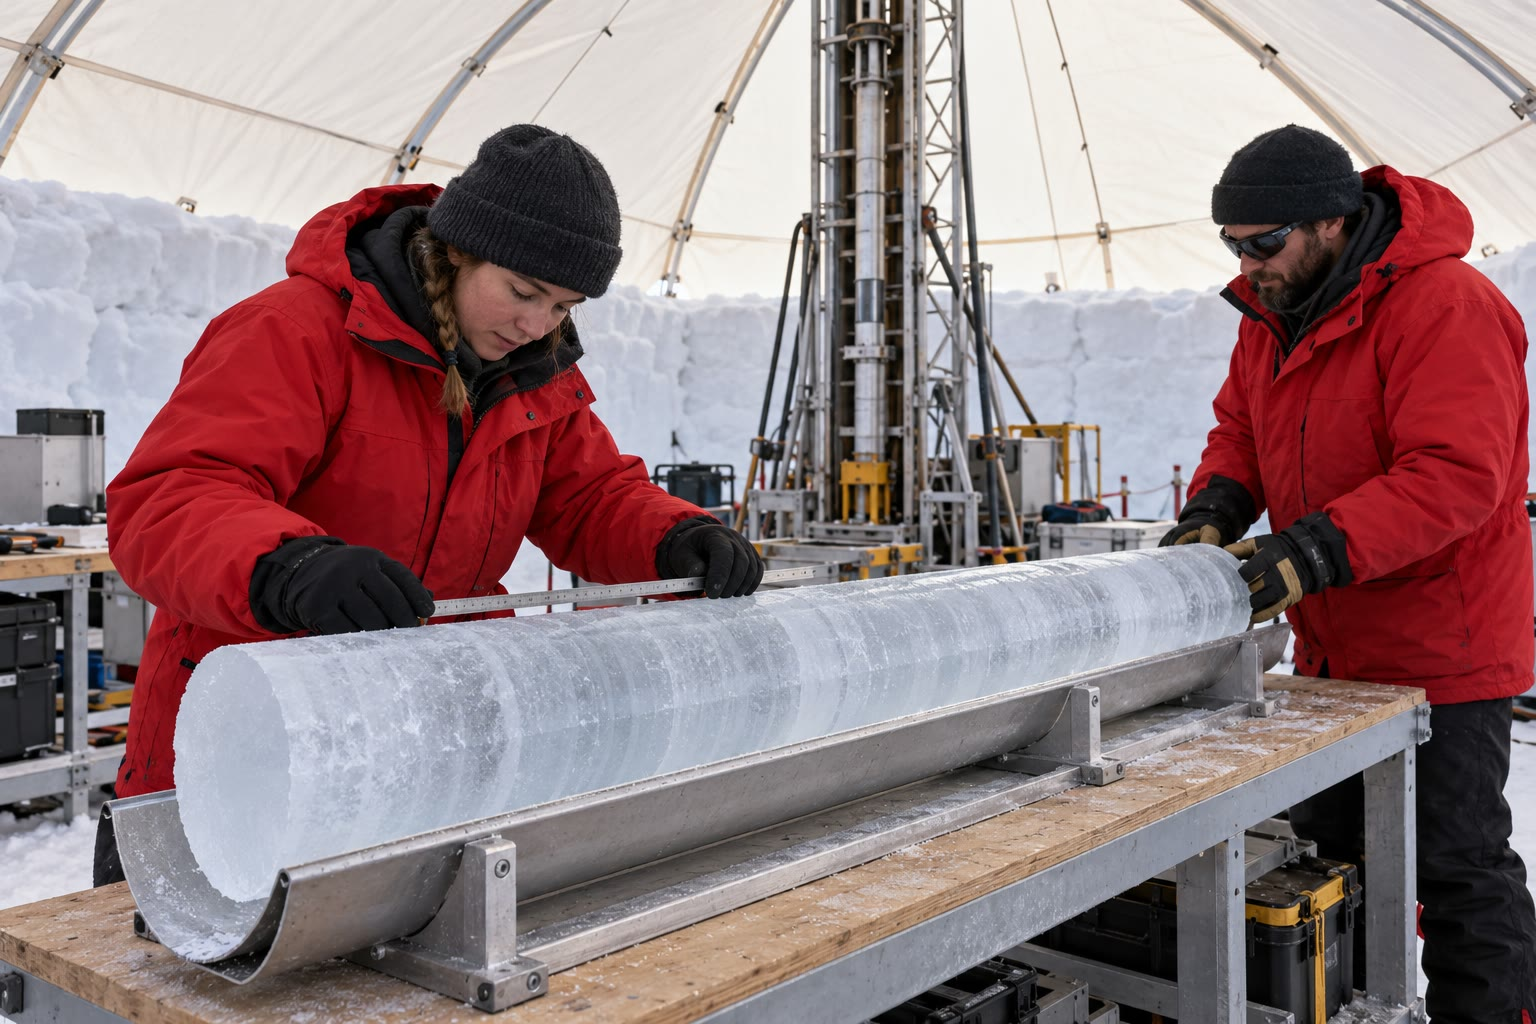
\includegraphics[width=\linewidth]{images/book5/ai/b3-ice-core-tent.jpg}

{\scriptsize Mesure d'une carotte de glace dans un berceau, dans une tente de forage posée sur une
calotte glaciaire, la tour de forage en arrière-plan (Illustration générée par IA.)}
\end{minipage}
\end{inthelab}

\section{Exercices}

\begin{exercise}[$\star$]\label{exo:b3:stable-isotopes:1}
Une calcite a $\delta^{18}\mathrm O = \qty{30.5}{\permil}$ et l'eau à partir de laquelle elle a cristallisé
\qty{-2.1}{\permil}, les deux étant exprimés par rapport au VSMOW. Calculer $\alpha$, $1000\ln\alpha$ et
$\Delta$. Quel écart sépare les deux dernières~?
\end{exercise}

\begin{exercise}[$\star$]\label{exo:b3:stable-isotopes:2}
Une station côtière de haute latitude a une température moyenne annuelle de
\qty{-25}{\celsius}. En utilisant les relations du chapitre pour de telles stations,
prévoir le $\delta^{18}\mathrm O$, le $\delta\mathrm D$ et l'\omterm{def:b3:stable-isotopes:d-excess}{excès en deutérium} de ses
précipitations.
\end{exercise}
% ledger: dansgaard64:effects

\begin{exercise}[$\star$]\label{exo:b3:stable-isotopes:3}
Dans un bassin, les carbonates ont $\delta^{13}\mathrm C = \qty{+1.0}{\permil}$ et la
matière organique \qty{-26.0}{\permil}. Avec des apports à \qty{-5}{\permil}, calculer
$f_{\mathrm{org}}$.
\end{exercise}
% ledger: planavsky22:forg

\begin{exercise}[$\star$]\label{exo:b3:stable-isotopes:4}
Une coquille de brachiopode présente $\Delta_{47} = \qty{0.600}{\permil}$. Avec l'étalonnage
du chapitre, à quelle température s'est-elle formée~?
\end{exercise}
% ledger: isogeochem:d47

\begin{exercise}[$\star\star$]\label{exo:b3:stable-isotopes:5}
La vapeur quitte l'océan à $\delta^{18}\mathrm O = \qty{-13}{\permil}$ et précipite
peu à peu avec un $\alpha = 1.0100$ constant. Quelle fraction en reste-t-il lorsque la
vapeur atteint \qty{-33}{\permil}~? Quel est le $\delta^{18}\mathrm O$ de la pluie
à ce moment-là~?
\end{exercise}
% ledger: white13c9:rayleigh

\begin{exercise}[$\star\star$]\label{exo:b3:stable-isotopes:6}
La neige à \qty{-40}{\permil} est comparée à de l'eau océanique à 0. Calculer $\alpha$,
$1000\ln\alpha$, $1000(\alpha - 1)$ et $\Delta$ entre elles. Laquelle des
approximations de la proposition est mise en défaut, et de combien~?
\end{exercise}

\begin{exercise}[$\star\star$]\label{exo:b3:stable-isotopes:7}
Un foraminifère a $\delta^{18}\mathrm O = \qty{+1.50}{\permil}$ (VPDB) et s'est formé dans
une eau à \qty{0.00}{\permil} (VSMOW). Calculer sa température de formation à l'aide de la
méthode du chapitre, et de combien une erreur de \qty{0.1}{\permil} sur la valeur de
l'eau modifie cette température.
\end{exercise}
% ledger: isogeochem:ko97

\begin{exercise}[$\star\star$]\label{exo:b3:stable-isotopes:8}
La pile benthique varie de \qty{1.77}{\permil} entre le présent et le dernier
maximum glaciaire. Retrancher la part due à l'effet de volume des glaces calculée dans le chapitre et
convertir le reste en variation de température des eaux profondes, à partir de la pente de
l'étalonnage de la calcite au voisinage de \qty{2}{\celsius}.
\end{exercise}
% ledger: data:lr04, white13c9:ice-volume, isogeochem:ko97

\begin{exercise}[$\star\star$]\label{exo:b3:stable-isotopes:9}
Une pyrite présente $\delta^{34}\mathrm S = \qty{10.0}{\permil}$ et $\delta^{33}\mathrm S =
\qty{8.2}{\permil}$. Calculer $\Delta^{33}\mathrm S$. Que nous apprend cette valeur sur
l'atmosphère au moment où la pyrite s'est formée~?
\end{exercise}
% ledger: white13c9:s-mif

\begin{exercise}[$\star\star\star$]\label{exo:b3:stable-isotopes:10}
Dans une condensation en système clos, la vapeur et tout le condensat formé restent
ensemble à l'équilibre. Montrer que la vapeur présente alors $R_v/R_{v,0} = 1/[f +
\alpha(1 - f)]$, et la comparer à la \omterm{prop:b3:stable-isotopes:rayleigh-distillation}{distillation de Rayleigh} pour $f = 0.2$ et
$\alpha = 1.01$.
\end{exercise}

\begin{exercise}[$\star\star\star$]\label{exo:b3:stable-isotopes:11}
À partir de l'estimation selon laquelle \qty{2000}{Gt} de carbone issu du méthane à
\qty{-60}{\permil} décale de \qty{-2.5}{\permil} le carbone échangeable,
déterminer la masse du réservoir qui en résulte, avec $\delta_0 = 0$. Avec cette masse, quelle quantité de
carbone organique à \qty{-25}{\permil} produit le même décalage~? Comparer avec la
fourchette publiée.
\end{exercise}
% ledger: dickens11:petm

\begin{exercise}[$\star\star\star$]\label{exo:b3:stable-isotopes:12}
Montrer que, le long d'un trajet de refroidissement, $\mathrm d\delta_v/\mathrm dT = (\alpha - 1)(1000 +
\delta_v)\,\mathrm d\ln e_s/\mathrm dT$. À \qty{-20}{\celsius}, où la
vapeur du modèle du chapitre présente $\delta^{18}\mathrm O = \qty{-49.1}{\permil}$
et la courbe de sublimation donne $\mathrm d\ln e_s/\mathrm dT =
\qty{0.0960}{K^{-1}}$, calculer cette pente.
\end{exercise}
% ledger: gkinis14:alpha-ice, iapws:melt-subl

\section{Problème~: le trajet d'une goutte de pluie jusqu'à Dome Ilse}

\begin{problem}[{Problème du week-end --- les isotopes de la neige le long d'une
traverse fictive, une paléotempérature et une excursion isotopique du carbone}]\label{pb:b3:stable-isotopes:1}
Une masse d'air quitte le bord d'une calotte glaciaire fictive à \qty{0}{\celsius}
avec une vapeur de $\delta^{18}\mathrm O = \qty{-20.0}{\permil}$ et $\delta\mathrm D =
\qty{-150}{\permil}$, et se refroidit à pression constante en progressant vers l'intérieur des terres.
La neige se forme à la station Coast à \qty{-10}{\celsius}, à Midway à
\qty{-20}{\celsius} et à Dome Ilse à \qty{-30}{\celsius}, lorsque la fraction
de vapeur restante vaut $f = 0.425$, $0.169$ et $0.0622$. Utiliser les
facteurs de fractionnement glace--vapeur du chapitre, constants sur chaque tronçon à la valeur
de leur température moyenne.
% ledger: gkinis14:alpha-ice, iapws:melt-subl, dansgaard64:effects, isogeochem:ko97, isogeochem:d47, white13c9:ice-volume, data:lr04, planavsky22:forg, dickens11:petm

\medskip\noindent\textbf{Partie I --- Distillation.}
\begin{enumerate}
\item Calculer $\alpha^{18}$ et $\alpha^{\mathrm D}$ à $-5$, $-10$, $-15$, $-20$,
$-25$ et \qty{-30}{\celsius} (cinq chiffres significatifs pour l'oxygène, quatre pour
le deutérium).
\item Calculer le $\delta^{18}\mathrm O$ de la vapeur à son arrivée à Coast.
\item Calculer celui de la neige tombée à Coast.
\item Refaire le calcul pour Midway (le rapport de $f$ sur le tronçon est $0.169/0.425$).
\item Refaire le calcul pour Dome Ilse.
\item Quelle fraction de l'oxygène 18 initial de la vapeur reste encore dans l'air
à Dome Ilse~?
\end{enumerate}

\medskip\noindent\textbf{Partie II --- Température et deutérium.}
\begin{enumerate}[resume]
\item Calculer la pente du $\delta^{18}\mathrm O$ de la neige en fonction de
la température de condensation, de la côte jusqu'à Dome Ilse.
\item Quelle température moyenne annuelle de surface la relation des stations
groenlandaises attribuerait-elle à la neige de Dome Ilse~? Pourquoi peut-elle
différer de \qty{-30}{\celsius}~?
\item Calculer de même le $\delta\mathrm D$ de la neige aux trois stations.
\item Calculer leur \omterm{def:b3:stable-isotopes:d-excess}{excès en deutérium}. Comment évolue-t-il à l'intérieur des terres~?
\item La neige de Dome Ilse se situe-t-elle sur la droite des eaux météoriques~? Qu'est-ce que le modèle
omet et que la formation réelle de la neige inclut~?
\end{enumerate}

\medskip\noindent\textbf{Partie III --- Un foraminifère au large.} Une
carotte sédimentaire prélevée au large fournit des foraminifères benthiques de \qty{3.25}{\permil}
VPDB au sommet et de \qty{5.02}{\permil} au dernier maximum glaciaire~; l'eau de fond
vaut aujourd'hui \qty{0.00}{\permil} VSMOW.
\begin{enumerate}[resume]
\item Calculer la température actuelle de l'eau de fond avec l'étalonnage
de la calcite.
\item Calculer la température glaciaire en supposant l'eau inchangée. Le
résultat est-il possible~?
\item Corriger l'eau glaciaire pour une baisse du niveau marin de \qty{125}{m} et
recalculer. Quel est le refroidissement glaciaire de l'eau de fond~?
\item Calculer le $\Delta_{47}$ attendu aux deux températures et leur
différence.
\item Pourquoi le thermomètre à \omterm{def:b3:stable-isotopes:clumped}{isotopes groupés} n'a-t-il pas besoin de la
composition de l'eau~?
\end{enumerate}

\medskip\noindent\textbf{Partie IV --- Une excursion du carbone.} Plus profondément dans la
carotte, des carbonates à \qty{+0.5}{\permil} sont interrompus par un
bref épisode à \qty{-3.0}{\permil}.
\begin{enumerate}[resume]
\item Avant l'excursion, avec $\delta_{\mathrm{in}} = \qty{-5}{\permil}$ et
$\Delta_B = \qty{-28}{\permil}$, calculer $f_{\mathrm{org}}$.
\item Prendre le réservoir de l'exercice 11, \qty{46000}{Gt} à 0. Quelle quantité de
carbone l'excursion exige-t-elle si la source est du méthane à \qty{-60}{\permil}~?
\item Et si c'est du carbone organique à \qty{-25}{\permil}~?
\item Et si c'est du carbone du manteau à \qty{-5}{\permil}~?
\item Quelle observation dans la même carotte pourrait aider à choisir entre les
sources~?
\item Donner le $\delta^{18}\mathrm O$ de la neige qui tombe à Dome Ilse.
\end{enumerate}
\end{problem}
